\documentclass[12pt,a4paper]{article}
\usepackage[polish]{babel}
\usepackage[T1]{fontenc}
\usepackage[utf8x]{inputenc}
\usepackage{hyperref}
\usepackage{url}
\usepackage{graphicx}
\usepackage{listings}
\usepackage{xcolor}

\addtolength{\hoffset}{-1.5cm}
\addtolength{\marginparwidth}{-1.5cm}
\addtolength{\textwidth}{3cm}
\addtolength{\voffset}{-1cm}
\addtolength{\textheight}{2.5cm}
\setlength{\topmargin}{0cm}
\setlength{\headheight}{0cm}

\lstset{
    numbers=left,
    breaklines=true,
    tabsize=2,
    basicstyle=\ttfamily,
}

\begin{document}
	
	\title{Systemy Sztucznej Inteligencji\\\small{dokumentacja projektu Unity Neural Network Car}}
	\author{Artur Bednarczyk, Dawid Grajewski, grupa A}
	\date{\today}

	\maketitle
	\newpage
	\section*{Część I}
	\subsection*{Opis programu}
	Tutaj, nasz super opis, jaki ten program jest cudowny i superowy. Nikt nie ma tak fajnego autka, które tak fajnie pędzi przez super fajny tor.
	Panie, inne autka tak nie pojadą jak nasze. Niżej jakiś normalny opis się zacznie;// \\
	
	Unity Nueral Network Car jest symulacją jazdy samochodu na torze. Samochód jest autonomiczny, co oznacza, że użytkownik nie musi go kontrolować, pojedzie sam. Samochód został nauczony jak jeździć dzięki specjalnie zaprojektowanej sieci neuronowej, dzięki czemu może jeździć po naszym torze nie rozbijając się na każdym zakręcie.
	\subsection*{Instrukcja obsługi}
	Magia dzieje się sama. Nie musisz tego znać.
	\subsection*{Dodatkowe informacje}
	Fajne, co nie? Tylko co mamy na myśli, mówiąc "Dodatkowe informacyje?"
	\newpage
	\section*{Część II}
	\subsection*{Opis działania} 
\subsubsection*{Sieć neuronowa}
Sieć neuronowa jest strukturą inspirowaną budową naturalnych neuronów, łączących je synaps oraz układów nerwowych. Wykorzystana w projekcie sieć jest wielowarstwową siecią jednokierunkową korzystającą z algorytmu propagacji wstecznej.
\subsubsection*{Budowa sieci}
Wykorzystana sieć składa się z trzech głównych warstw.
\begin{itemize}
	\item Warstwa wejścia.
	\item Warstwy ukryte.
	\item Warstwa wyjścia.
\end{itemize}
\paragraph*{Warstwa wejścia} Każdy neuron tej warstwy przekazuje do warstwy ukrytej początkowe wartości.
\paragraph*{Warstwy ukryte} Tutaj dzieje się wszystko co najważniejsze. Neurony mają przypisane wagi, które początkowo są losowe. W ramach uczenia się, wagi są dostosowywane tak, aby rezultat końcowy był jak najbliżej spodziewanego.
\paragraph*{Warstwa wyjścia} To tutaj nauczona już sieć daje nam wynik.
\subsubsection*{Uczenie sieci}
Uczenie sieci jest realizowane poprzez podanie jej zestawu danych wejściowych oraz spodziewanych wyników. W tym projekcie wykorzystano metody takie jak:
\begin{itemize}
\item Propagacja Wsteczna
\item Biases
\item Momentum
\item Współczynnik uczenia
\end{itemize}
\paragraph*{Propagacja wsteczna} tutaj trochę o tym... będą wzory, będą opisy, będzie fajnie. 
\paragraph*{Biases} tutaj trochę o tym...
\paragraph*{Momentum} tutaj trochę o tym...
\paragraph*{Współczynnik uczenia} tutaj trochę o tym...
\subsubsection*{Funkcja Aktywacji}
Wartość wyjścia neuronów jest oblicznaa za pomocą funkcji aktywacji. W tym projekcie została użyta funkcja sigmoidalna:
$$ S(x) = \frac{1}{1+e^{-x}} = \frac{e^x}{e^x+1} $$

	
	PROPAGACJA WSTECZNA \\
	https://mattmazur.com/2015/03/17/a-step-by-step-backpropagation-example/ \\
	xD\\
	\subsection*{Algorytm}
	mile widziany pseudokod z użyciem biblioteki \LaTeX
	\\
	\\
	pseudo kod czego naszego AI tutaj sie da; o ile da rade te wszystkie rzeczy w coś krótkiego zwinąć, bo inaczej jest w tym sens, skoro cały kod będzie niżej?\\
	\\
	Jak to nie będzie zbyt ogromne, to mogę zrobić ładny(jak się uda) schemat blokowy.
	\subsection*{Bazy danych}
	Należy pokazać przykładowe dane, które były wykorzystywane podczas uczenia klasyfikatorów.
	\\
	Czyli te 120 wierszy czy ile tego tam mamy? Czy wystarczy mu pokazać, że mamy dane w takiej formie i wkleić kilka wierszy tego i dać trzy kropki, o takie "...".
	\subsection*{Implementacja}
	Opis, zasada i działanie programu ze względu na podział na pliki, nastepnie	funkcje programu wraz ze szczegółowym opisem działania
	\begin{verbatim}
	proszę zwrócić uwagę na wychodzenie poza obszar kartki.
	
	No spoko, ja tu dopiljnuje, żeby wyglądało po ludzku.
	\end{verbatim}
	\subsection*{Testy}
	Tutaj powinna pojawić się analiza uzyskanych wyników oraz wykresy/pomiary.
	
	No lekko, tutaj wleci super wykres nakodzony w pytonie. \\
	%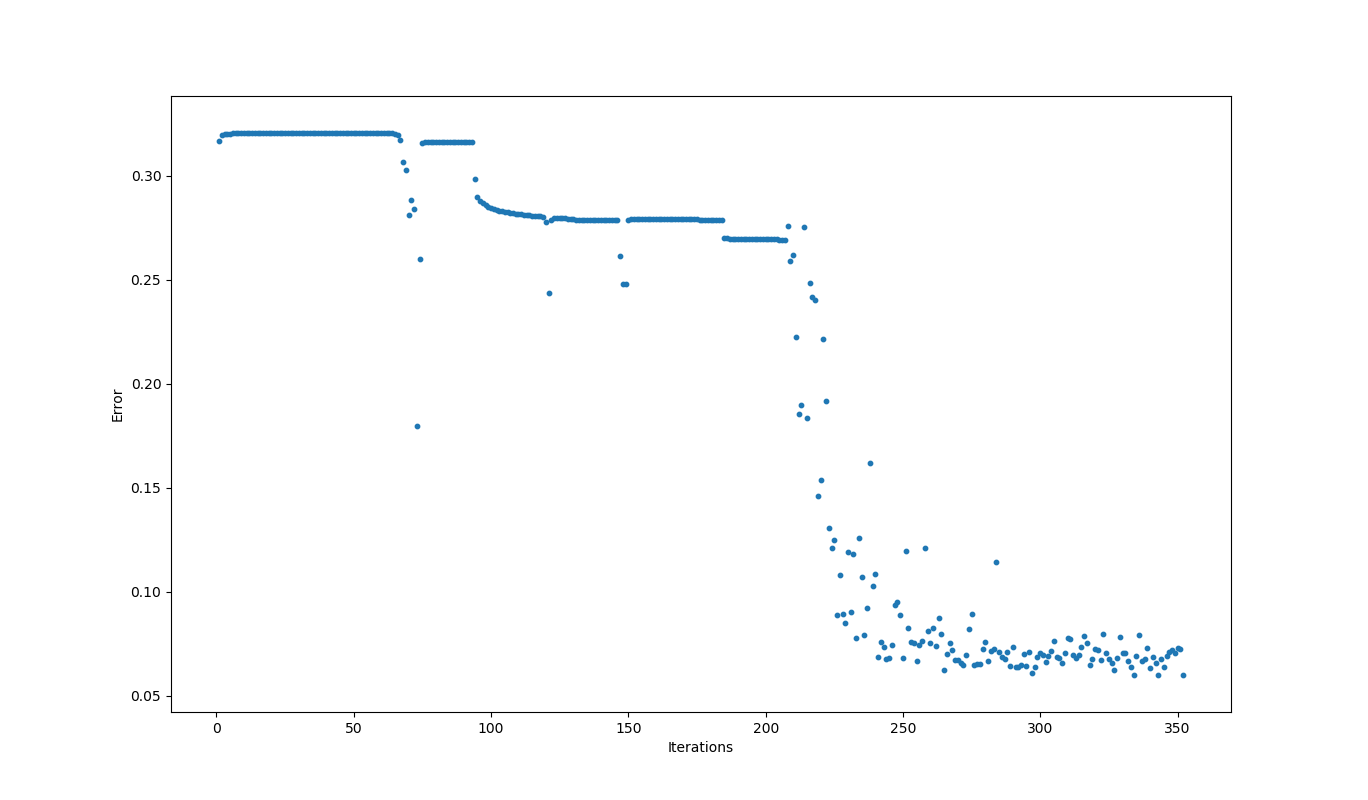
\includegraphics[scale=0.5]{supa_wykres}
	\newpage
	\section*{Pełen kod aplikacji}
	tutaj wklejamy pełen kod.\\ Dalej nie rozumiem sensu tego punktu. ale niech będzie. Pewnie wszystko będzie ważyło trochę zbyt dużo, żeby to wrzucić na platformę xD
	\section*{Neuron}
	\begin{lstlisting}
public class Neuron
{
	#region -- Properties --
	public Guid Id { get; set; }
	public List<Synapse> InputSynapses { get; set; }
	public List<Synapse> OutputSynapses { get; set; }
	public double Bias { get; set; }
	public double BiasDelta { get; set; }
	public double Gradient { get; set; }
	public double Value { get; set; }
	#endregion

	#region -- Constructors --
	public Neuron()
	{
		Id = Guid.NewGuid();
		InputSynapses = new List<Synapse>();
		OutputSynapses = new List<Synapse>();
		Bias = Network.GetRandom();
	}

	public Neuron(IEnumerable<Neuron> inputNeurons) : this()
	{
		foreach (var inputNeuron in inputNeurons)
		{
			var synapse = new Synapse(inputNeuron, this);
			inputNeuron.OutputSynapses.Add(synapse);
			InputSynapses.Add(synapse);
		}
	}
	#endregion

	#region -- Values & Weights --
	public virtual double CalculateValue()
	{
		return Value = Sigmoid.Output(InputSynapses.Sum(a => a.Weight * a.InputNeuron.Value) + Bias);
	}

	public double CalculateError(double target)
	{
		return target - Value;
	}

	public double CalculateGradient(double? target = null)
	{
		if (target == null)
			return Gradient = OutputSynapses.Sum(a => a.OutputNeuron.Gradient * a.Weight) * Sigmoid.Derivative(Value);

		return Gradient = CalculateError(target.Value) * Sigmoid.Derivative(Value);
	}

	public void UpdateWeights(double learnRate, double momentum)
	{
		var prevDelta = BiasDelta;
		BiasDelta = learnRate * Gradient;
		Bias += BiasDelta + momentum * prevDelta;

		foreach (var synapse in InputSynapses)
		{
			prevDelta = synapse.WeightDelta;
			synapse.WeightDelta = learnRate * Gradient * synapse.InputNeuron.Value;
			synapse.Weight += synapse.WeightDelta + momentum * prevDelta;
		}
	}
	#endregion
}
	\end{lstlisting}
	
	\section*{Synapse}
	\begin{lstlisting}
	public class Synapse
	{
		#region -- Properties --
		public Guid Id { get; set; }
		public Neuron InputNeuron { get; set; }
		public Neuron OutputNeuron { get; set; }
		public double Weight { get; set; }
		public double WeightDelta { get; set; }
		#endregion

		#region -- Constructor --
		public Synapse() { }

		public Synapse(Neuron inputNeuron, Neuron outputNeuron)
		{
			Id = Guid.NewGuid();
			InputNeuron = inputNeuron;
			OutputNeuron = outputNeuron;
			Weight = Network.GetRandom();
		}
		#endregion
	}
	\end{lstlisting}
	
	\section*{Network}
	\begin{lstlisting}
	public class Network
	{
		#region -- Properties --
		public double LearnRate { get; set; }
		public double Momentum { get; set; }
		public List<Neuron> InputLayer { get; set; }
		public List<List<Neuron>> HiddenLayers { get; set; }
		public List<Neuron> OutputLayer { get; set; }
        public bool ShowIterationError { get; set; }
		#endregion

		#region -- Globals --
		private static readonly Random Random = new Random();
		#endregion

		#region -- Constructor --
		public Network()
		{
			LearnRate = 0;
			Momentum = 0;
			InputLayer = new List<Neuron>();
			HiddenLayers = new List<List<Neuron>>();
			OutputLayer = new List<Neuron>();
		}

        public Network(int inputSize, int[] hiddenSizes, int outputSize, double? learnRate = null, double? momentum = null, bool showIterationError = false)
		{
            ShowIterationError = showIterationError;
			LearnRate = learnRate ?? .4;
			Momentum = momentum ?? .9;
			InputLayer = new List<Neuron>();
			HiddenLayers = new List<List<Neuron>>();
			OutputLayer = new List<Neuron>();

			for (var i = 0; i < inputSize; i++)
				InputLayer.Add(new Neuron());

			var firstHiddenLayer = new List<Neuron>();
			for (var i = 0; i < hiddenSizes[0]; i++)
				firstHiddenLayer.Add(new Neuron(InputLayer));

			HiddenLayers.Add(firstHiddenLayer);

			for (var i = 1; i < hiddenSizes.Length; i++)
			{
				var hiddenLayer = new List<Neuron>();
				for (var j = 0; j < hiddenSizes[i]; j++)
					hiddenLayer.Add(new Neuron(HiddenLayers[i - 1]));
				HiddenLayers.Add(hiddenLayer);
			}

			for (var i = 0; i < outputSize; i++)
				OutputLayer.Add(new Neuron(HiddenLayers.Last()));
		}
		#endregion

		#region -- Training --
		public void Train(List<DataSet> dataSets, int numEpochs)
		{
			for (var i = 0; i < numEpochs; i++)
			{
				foreach (var dataSet in dataSets)
				{
					ForwardPropagate(dataSet.Values);
					BackPropagate(dataSet.Targets);
				}
			}
		}

		public void Train(List<DataSet> dataSets, double minimumError)
		{
			var error = 1.0;
			var numEpochs = 0;

			while (error > minimumError && numEpochs < int.MaxValue)
			{
				var errors = new List<double>();
				foreach (var dataSet in dataSets)
				{
					ForwardPropagate(dataSet.Values);
					BackPropagate(dataSet.Targets);
					errors.Add(CalculateError(dataSet.Targets));
				}
				error = errors.Average();
                numEpochs++;

                if(ShowIterationError)
                    Console.WriteLine(error);
			}
		}

		private void ForwardPropagate(params double[] inputs)
		{
			var i = 0;
			InputLayer.ForEach(a => a.Value = inputs[i++]);
			HiddenLayers.ForEach(a => a.ForEach(b => b.CalculateValue()));
			OutputLayer.ForEach(a => a.CalculateValue());
		}

		private void BackPropagate(params double[] targets)
		{
			var i = 0;
			OutputLayer.ForEach(a => a.CalculateGradient(targets[i++]));
			HiddenLayers.Reverse();
			HiddenLayers.ForEach(a => a.ForEach(b => b.CalculateGradient()));
			HiddenLayers.ForEach(a => a.ForEach(b => b.UpdateWeights(LearnRate, Momentum)));
			HiddenLayers.Reverse();
			OutputLayer.ForEach(a => a.UpdateWeights(LearnRate, Momentum));
		}

		public double[] Compute(params double[] inputs)
		{
			ForwardPropagate(inputs);
			return OutputLayer.Select(a => a.Value).ToArray();
		}

		private double CalculateError(params double[] targets)
		{
			var i = 0;
			return OutputLayer.Sum(a => Math.Abs(a.CalculateError(targets[i++])));
		}
		#endregion

		#region -- Helpers --
		public static double GetRandom()
		{
			return 2 * Random.NextDouble() - 1;
		}
		#endregion
	}

	#region -- Enum --
	public enum TrainingType
	{
		Epoch,
		MinimumError
	}
	#endregion
	\end{lstlisting}
	
	\section*{Sigmoid}
	\begin{lstlisting}
	public static class Sigmoid
	{
		public static double Output(double x)
		{
			return x < -45.0 ? 0.0 : x > 45.0 ? 1.0 : 1.0 / (1.0 + Math.Exp(-x));
		}

		public static double Derivative(double x)
		{
			return x * (1 - x);
		}
	}
	\end{lstlisting}
	
	\section*{Dataset}
	\begin{lstlisting}
	public class DataSet
	{
		#region -- Properties --
		public double[] Values { get; set; }
		public double[] Targets { get; set; }
		#endregion

		#region -- Constructor --
		public DataSet(double[] values, double[] targets)
		{
			Values = values;
			Targets = targets;
		}
		#endregion
	}
	\end{lstlisting}
	
	\section*{ExportHelper}
	\begin{lstlisting}
	public static class ExportHelper
	{
        public static void ExportNetwork(Network network, string filename, ISerializer serializer)
        {
            var dn = GetHelperNetwork(network);

            serializer.Serialize(dn, filename);
        }

		private static HelperNetwork GetHelperNetwork(Network network)
		{
			var hn = new HelperNetwork
			{
				LearnRate = network.LearnRate,
				Momentum = network.Momentum
			};

			//Input Layer
			foreach (var n in network.InputLayer)
			{
				var neuron = new HelperNeuron
				{
					Id = n.Id,
					Bias = n.Bias,
					BiasDelta = n.BiasDelta,
					Gradient = n.Gradient,
					Value = n.Value
				};

				hn.InputLayer.Add(neuron);

				foreach (var synapse in n.OutputSynapses)
				{
					var syn = new HelperSynapse
					{
						Id = synapse.Id,
						OutputNeuronId = synapse.OutputNeuron.Id,
						InputNeuronId = synapse.InputNeuron.Id,
						Weight = synapse.Weight,
						WeightDelta = synapse.WeightDelta
					};

					hn.Synapses.Add(syn);
				}
			}

			//Hidden Layer
			foreach (var l in network.HiddenLayers)
			{
				var layer = new List<HelperNeuron>();

				foreach (var n in l)
				{
					var neuron = new HelperNeuron
					{
						Id = n.Id,
						Bias = n.Bias,
						BiasDelta = n.BiasDelta,
						Gradient = n.Gradient,
						Value = n.Value
					};

					layer.Add(neuron);

					foreach (var synapse in n.OutputSynapses)
					{
						var syn = new HelperSynapse
						{
							Id = synapse.Id,
							OutputNeuronId = synapse.OutputNeuron.Id,
							InputNeuronId = synapse.InputNeuron.Id,
							Weight = synapse.Weight,
							WeightDelta = synapse.WeightDelta
						};

						hn.Synapses.Add(syn);
					}
				}

				hn.HiddenLayers.Add(layer);
			}

			//Output Layer
			foreach (var n in network.OutputLayer)
			{
				var neuron = new HelperNeuron
				{
					Id = n.Id,
					Bias = n.Bias,
					BiasDelta = n.BiasDelta,
					Gradient = n.Gradient,
					Value = n.Value
				};

				hn.OutputLayer.Add(neuron);

				foreach (var synapse in n.OutputSynapses)
				{
					var syn = new HelperSynapse
					{
						Id = synapse.Id,
						OutputNeuronId = synapse.OutputNeuron.Id,
						InputNeuronId = synapse.InputNeuron.Id,
						Weight = synapse.Weight,
						WeightDelta = synapse.WeightDelta
					};

					hn.Synapses.Add(syn);
				}
			}

			return hn;
		}
	}
	\end{lstlisting}
	
	\section*{ImportHelper}
	\begin{lstlisting}
	public static class ImportHelper
	{
        public static Network ImportNetwork(string filename, ISerializer serializer)
        {
            var dn = GetHelperNetwork(filename, serializer);
            if (dn == null) return null;

            var network = new Network();
            var allNeurons = new List<Neuron>();

            network.LearnRate = dn.LearnRate;
            network.Momentum = dn.Momentum;

            //Input Layer
            foreach (var n in dn.InputLayer)
            {
                var neuron = new Neuron
                {
                    Id = n.Id,
                    Bias = n.Bias,
                    BiasDelta = n.BiasDelta,
                    Gradient = n.Gradient,
                    Value = n.Value
                };

                network.InputLayer.Add(neuron);
                allNeurons.Add(neuron);
            }

            //Hidden Layers
            foreach (var layer in dn.HiddenLayers)
            {
                var neurons = new List<Neuron>();
                foreach (var n in layer)
                {
                    var neuron = new Neuron
                    {
                        Id = n.Id,
                        Bias = n.Bias,
                        BiasDelta = n.BiasDelta,
                        Gradient = n.Gradient,
                        Value = n.Value
                    };

                    neurons.Add(neuron);
                    allNeurons.Add(neuron);
                }

                network.HiddenLayers.Add(neurons);
            }

            //Export Layer
            foreach (var n in dn.OutputLayer)
            {
                var neuron = new Neuron
                {
                    Id = n.Id,
                    Bias = n.Bias,
                    BiasDelta = n.BiasDelta,
                    Gradient = n.Gradient,
                    Value = n.Value
                };

                network.OutputLayer.Add(neuron);
                allNeurons.Add(neuron);
            }

            //Synapses
            foreach (var syn in dn.Synapses)
            {
                var synapse = new Synapse { Id = syn.Id };
                var inputNeuron = allNeurons.First(x => x.Id == syn.InputNeuronId);
                var outputNeuron = allNeurons.First(x => x.Id == syn.OutputNeuronId);
                synapse.InputNeuron = inputNeuron;
                synapse.OutputNeuron = outputNeuron;
                synapse.Weight = syn.Weight;
                synapse.WeightDelta = syn.WeightDelta;

                inputNeuron.OutputSynapses.Add(synapse);
                outputNeuron.InputSynapses.Add(synapse);
            }

            return network;
        }

        private static HelperNetwork GetHelperNetwork(string filename, ISerializer serializer)
        {
            return serializer.Deserialize(filename);
        }

    }
	\end{lstlisting}
	
	\section*{Helpers}
	\begin{lstlisting}
	public class HelperNetwork
	{
		public double LearnRate { get; set; }
		public double Momentum { get; set; }
		public List<HelperNeuron> InputLayer { get; set; }
		public List<List<HelperNeuron>> HiddenLayers { get; set; }
		public List<HelperNeuron> OutputLayer { get; set; }
		public List<HelperSynapse> Synapses { get; set; }

		public HelperNetwork()
		{
			InputLayer = new List<HelperNeuron>();
			HiddenLayers = new List<List<HelperNeuron>>();
			OutputLayer = new List<HelperNeuron>();
			Synapses = new List<HelperSynapse>();
		}
	}

	public class HelperNeuron
	{
		public Guid Id { get; set; }
		public double Bias { get; set; }
		public double BiasDelta { get; set; }
		public double Gradient { get; set; }
		public double Value { get; set; }
	}

	public class HelperSynapse
	{
		public Guid Id { get; set; }
		public Guid OutputNeuronId { get; set; }
		public Guid InputNeuronId { get; set; }
		public double Weight { get; set; }
		public double WeightDelta { get; set; }
	}
	\end{lstlisting}
	
	\section*{Serializer}
	\begin{lstlisting}
	public interface ISerializer
{
    void Serialize(HelperNetwork network, string filename);
    HelperNetwork Deserialize(string filename);
}

public class XmlSerializer : ISerializer
{
    public HelperNetwork Deserialize(string filename)
    {
        using (var reader = new StreamReader(filename))
        {
            var serializer = new System.Xml.Serialization.XmlSerializer(typeof(HelperNetwork));
            return serializer.Deserialize(reader) as HelperNetwork;
        }
    }

    public void Serialize(HelperNetwork network, string filename)
    {
        using (var writer = new StreamWriter(filename))
        {
            var serializer = new System.Xml.Serialization.XmlSerializer(network.GetType());
            serializer.Serialize(writer, network);
        }
    }
}
	\end{lstlisting}
	
	\section*{CarController}
	\begin{lstlisting}
	public abstract class CarController : MonoBehaviour
{
    [Header("Steering")]
    public int MovementSpeed;
    public int RotationSpeed;

    [Header("Sensors")]
    public float SensorLength;
    public float SensorAngle;

    public float DistanceToLeftWall { get; private set; }
    public float DistanceToRightWall { get; private set; }

	
	// Update is called once per frame
	protected virtual void Update () {
        getDistanceToWalls();
    }

    public void MoveForward()
    {
        transform.position += transform.forward * MovementSpeed * Time.deltaTime;
    }

    public void TurnLeft()
    {
        transform.Rotate(Vector3.down * Time.deltaTime * RotationSpeed);
    }

    public void TurnRight()
    {
        transform.Rotate(Vector3.up * Time.deltaTime * RotationSpeed);
    }

    private void getDistanceToWalls()
    {
        RaycastHit leftHit;
        RaycastHit rightHit;
        Vector3 leftSensorStartPosition = transform.position;
        Vector3 rightSensorStartPosition = transform.position;

        if (Physics.Raycast(leftSensorStartPosition, Quaternion.AngleAxis(-SensorAngle, transform.up) * transform.forward, out leftHit, SensorLength))
        {
            DistanceToLeftWall = Vector3.Distance(leftSensorStartPosition, leftHit.point);
            Debug.DrawLine(leftSensorStartPosition, leftHit.point);
        }

        if (Physics.Raycast(rightSensorStartPosition, Quaternion.AngleAxis(SensorAngle, transform.up) * transform.forward, out rightHit, SensorLength))
        {
            DistanceToRightWall = Vector3.Distance(rightSensorStartPosition, rightHit.point);
            Debug.DrawLine(rightSensorStartPosition, rightHit.point);
        }
    }

    void OnTriggerEnter(Collider other)
    {
        SceneManager.LoadScene(SceneManager.GetActiveScene().name);
    }
}
	\end{lstlisting}
	
	\section*{AutonomicCarController}
	\begin{lstlisting}
public class AutonomicCarController : CarController
{
    [Header("Neural network holder")]
    // Odwolanie do obiektu z siecia neuronowa
    public BrainController Brain;

    private const double turnRightCondition = 2f / 3f;
    private const double turnLeftCondition = 1f / 3f;

    // Update is called once per frame
    protected override void Update ()
    {
        base.Update();
        MoveForward();
        steer();
	}

    private void steer()
    {
        neuralNetworkSteer();
    }

    private void simpleSteer()
    {
        var difference = DistanceToRightWall - DistanceToLeftWall;
        makeDecision(difference, 1, -1);
    }

    private void neuralNetworkSteer()
    {
        var networkOutput = Brain.Compute(DistanceToLeftWall, DistanceToRightWall);
        makeDecision(networkOutput, turnRightCondition, turnLeftCondition);
    }

    private void makeDecision(double value, double turnRightCondition, double turnLeftCondition)
    {
        if (value > turnRightCondition)
            TurnRight();
        else if (value < turnLeftCondition)
            TurnLeft();
    }
}
	\end{lstlisting}
	
	\section*{ManualCarController}
	\begin{lstlisting}
public class ManualCarController : CarController
{
    [Header("Steering")]
    public KeyCode UpKey = KeyCode.W;
    public KeyCode RightKey = KeyCode.D;
    public KeyCode LeftKey = KeyCode.A;

    [Header("Learning Data")]
    public bool CollectLearningData;
    public double CollectiongDataInterval;
    public string LearnignDataFileName;

    private double elapsedTimeSinceLastCollection = 0;
    private const char learningFileDelimiter = ';';


    // Update is called once per frame
    protected override void Update ()
    {
        base.Update();

        move();

        if (CollectLearningData)
        {
            elapsedTimeSinceLastCollection += Time.deltaTime;

            if (elapsedTimeSinceLastCollection >= CollectiongDataInterval)
            {
                collectLearningdata();
                elapsedTimeSinceLastCollection = 0;
            }
        }
    }

    private void move()
    {
        if (Input.GetKey(UpKey))
        {
            MoveForward();
        }

        if (Input.GetKey(RightKey))
        {
            TurnRight();
        }
        if (Input.GetKey(LeftKey))
        {
            TurnLeft();
        }
    }

    private void collectLearningdata()
    {
        using (var writer = File.AppendText(LearnignDataFileName))
        {
            var expectedOutput = Sigmoid.Output(DistanceToRightWall - DistanceToLeftWall);
            Debug.Log(expectedOutput);
            writer.WriteLine(string.Format("{0}{3}{1}{3}{2}", DistanceToLeftWall, DistanceToRightWall, expectedOutput, learningFileDelimiter));
            Debug.Log(DistanceToLeftWall + " " + DistanceToRightWall + " " + expectedOutput);
        }
    }
}
	\end{lstlisting}
	
	\section*{BrainController}
	\begin{lstlisting}
public class BrainController : MonoBehaviour
{
    [Header("Learned")]
    public string LearnedNetworkFileName;

    [Header("Learning")]
    public bool TrainOnInit;
    public string LearningFileName;
    public double MaxError;

    private const char _learningFileDelimiter = ';';

    public NeuralNetwork.NetworkModels.Network NeuralNetwork { get; private set; }

	// Use this for initialization
	void Start ()
    {
        if (TrainOnInit)
            Train();
        else
            Load();
    }

    /// <summary>
    /// Wyciaga z sieci wynik na podstawie odleglosci od scian
    /// </summary>
    /// <param name="distanceToLeftWall"></param>
    /// <param name="distanceToRightWall"></param>
    /// <returns></returns>
    public double Compute(double distanceToLeftWall, double distanceToRightWall)
    {
        return NeuralNetwork.Compute(new double[] { distanceToLeftWall, distanceToRightWall })[0];
    }

    public void Train()
    {
        NeuralNetwork.Train(getDatasets(), MaxError);
    }

    public void Save()
    {
        ExportHelper.ExportNetwork(NeuralNetwork, LearnedNetworkFileName, new XmlSerializer());
    }

    public void Load()
    {
        NeuralNetwork = ImportHelper.ImportNetwork(LearnedNetworkFileName, new XmlSerializer());
    }

    public void TestNetwork()
    {
        double l = 14;
        double r = 14;
        Debug.Log (NeuralNetwork.Compute(new double[] { l, r })[0] );

        l = 20;
        r = 10;
        Debug.Log(NeuralNetwork.Compute(new double[] { l, r })[0]);

        l = 10.72468;
        r = 42.37657;
        Debug.Log(NeuralNetwork.Compute(new double[] { l, r })[0]);
    }

    private List<DataSet> getDatasets()
    {
        var result = new List<DataSet>();

        using (var reader = new StreamReader(LearningFileName))
        {
            while(!reader.EndOfStream)
            {
                var elements = reader.ReadLine().Split(_learningFileDelimiter);
                var dataset = new DataSet(new double[] { double.Parse(elements[0]), double.Parse(elements[1]) }, new double[] { double.Parse(elements[2]) });
                result.Add(dataset);
            }
        }

        return result;
    }
}
	\end{lstlisting}
\end{document}
